\PassOptionsToPackage{unicode=true}{hyperref} % options for packages loaded elsewhere
\PassOptionsToPackage{hyphens}{url}
%
\documentclass[12pt,]{article}
\usepackage{lmodern}
\usepackage{amssymb,amsmath}
\usepackage{ifxetex,ifluatex}
\usepackage{fixltx2e} % provides \textsubscript
\ifnum 0\ifxetex 1\fi\ifluatex 1\fi=0 % if pdftex
  \usepackage[T1]{fontenc}
  \usepackage[utf8]{inputenc}
  \usepackage{textcomp} % provides euro and other symbols
\else % if luatex or xelatex
  \usepackage{unicode-math}
  \defaultfontfeatures{Ligatures=TeX,Scale=MatchLowercase}
    \setmainfont[]{Times New Roman}
\fi
% use upquote if available, for straight quotes in verbatim environments
\IfFileExists{upquote.sty}{\usepackage{upquote}}{}
% use microtype if available
\IfFileExists{microtype.sty}{%
\usepackage[]{microtype}
\UseMicrotypeSet[protrusion]{basicmath} % disable protrusion for tt fonts
}{}
\IfFileExists{parskip.sty}{%
\usepackage{parskip}
}{% else
\setlength{\parindent}{0pt}
\setlength{\parskip}{6pt plus 2pt minus 1pt}
}
\usepackage{hyperref}
\hypersetup{
            pdftitle={Changes on the Elwha River During Dam Removal},
            pdfauthor={Kathleen Mason},
            pdfborder={0 0 0},
            breaklinks=true}
\urlstyle{same}  % don't use monospace font for urls
\usepackage[margin=2.54cm]{geometry}
\usepackage{graphicx,grffile}
\makeatletter
\def\maxwidth{\ifdim\Gin@nat@width>\linewidth\linewidth\else\Gin@nat@width\fi}
\def\maxheight{\ifdim\Gin@nat@height>\textheight\textheight\else\Gin@nat@height\fi}
\makeatother
% Scale images if necessary, so that they will not overflow the page
% margins by default, and it is still possible to overwrite the defaults
% using explicit options in \includegraphics[width, height, ...]{}
\setkeys{Gin}{width=\maxwidth,height=\maxheight,keepaspectratio}
\setlength{\emergencystretch}{3em}  % prevent overfull lines
\providecommand{\tightlist}{%
  \setlength{\itemsep}{0pt}\setlength{\parskip}{0pt}}
\setcounter{secnumdepth}{5}
% Redefines (sub)paragraphs to behave more like sections
\ifx\paragraph\undefined\else
\let\oldparagraph\paragraph
\renewcommand{\paragraph}[1]{\oldparagraph{#1}\mbox{}}
\fi
\ifx\subparagraph\undefined\else
\let\oldsubparagraph\subparagraph
\renewcommand{\subparagraph}[1]{\oldsubparagraph{#1}\mbox{}}
\fi

% set default figure placement to htbp
\makeatletter
\def\fps@figure{htbp}
\makeatother

\usepackage{etoolbox}
\makeatletter
\providecommand{\subtitle}[1]{% add subtitle to \maketitle
  \apptocmd{\@title}{\par {\large #1 \par}}{}{}
}
\makeatother

\title{Changes on the Elwha River During Dam Removal}
\providecommand{\subtitle}[1]{}
\subtitle{\url{https://github.com/kfm20/DataProject_ElwhaRiver.git}}
\author{Kathleen Mason}
\date{}

\begin{document}
\maketitle

\newpage
\tableofcontents 
\newpage
\listoftables 
\newpage
\listoffigures 
\newpage

\hypertarget{rationale-and-research-questions}{%
\section{Rationale and Research
Questions}\label{rationale-and-research-questions}}

\newpage

\hypertarget{dataset-information}{%
\section{Dataset Information}\label{dataset-information}}

\newpage

\hypertarget{exploratory-analysis}{%
\section{Exploratory Analysis}\label{exploratory-analysis}}

An initial exploratory analysis is conducted to see general trends in
data related to water and sediment discharge, and suspended
concentrations in Elwha River during and after the dam removal process.
Daily water discharge from the river, \emph{Figure 1}, appears to have
higher peaks of discharge in 2015 and 2016, the years after the dam
removal project was complete. Embedding the dates involved with the dam
removal process, such as start of removal, and completion of each dam
removal will help differentiate differences in discharge related to more
open flows with dams removed. This data might need to be looked at a
different scale, instead of daily, maybe monthly averages will show a
different relationship, or a similar one at a different magnitude.

\begin{figure}
\centering
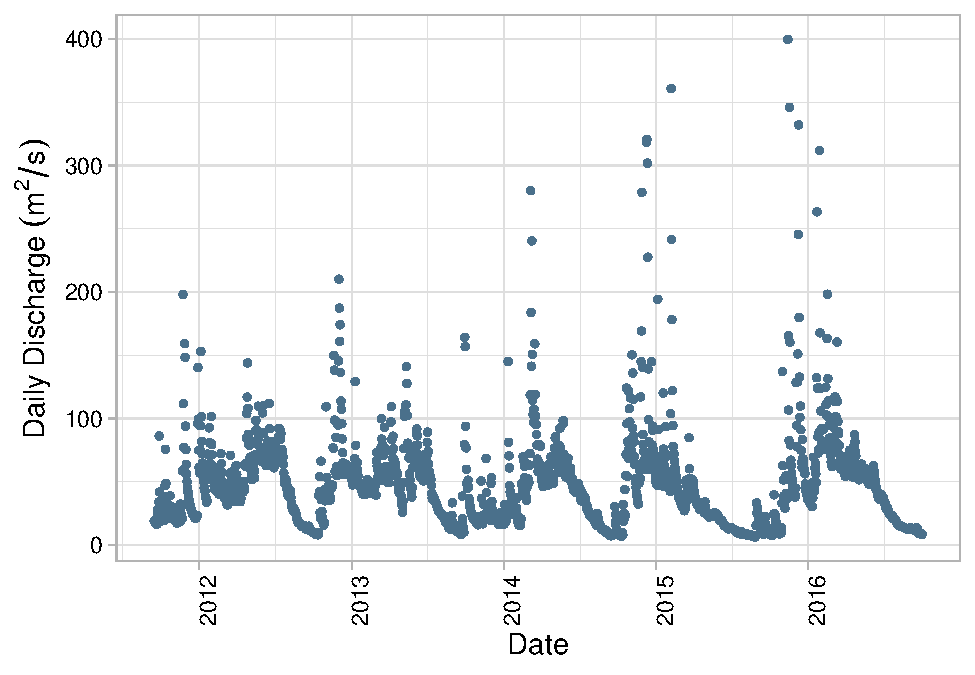
\includegraphics{Mason_ENV872_ProjectFinal_files/figure-latex/Exploratory Analysis Figure 1-1.pdf}
\caption{Daily water discahrge of the Elwha River, WA, from September
15, 2011 to September 30, 2016.}
\end{figure}

\begin{figure}
\centering
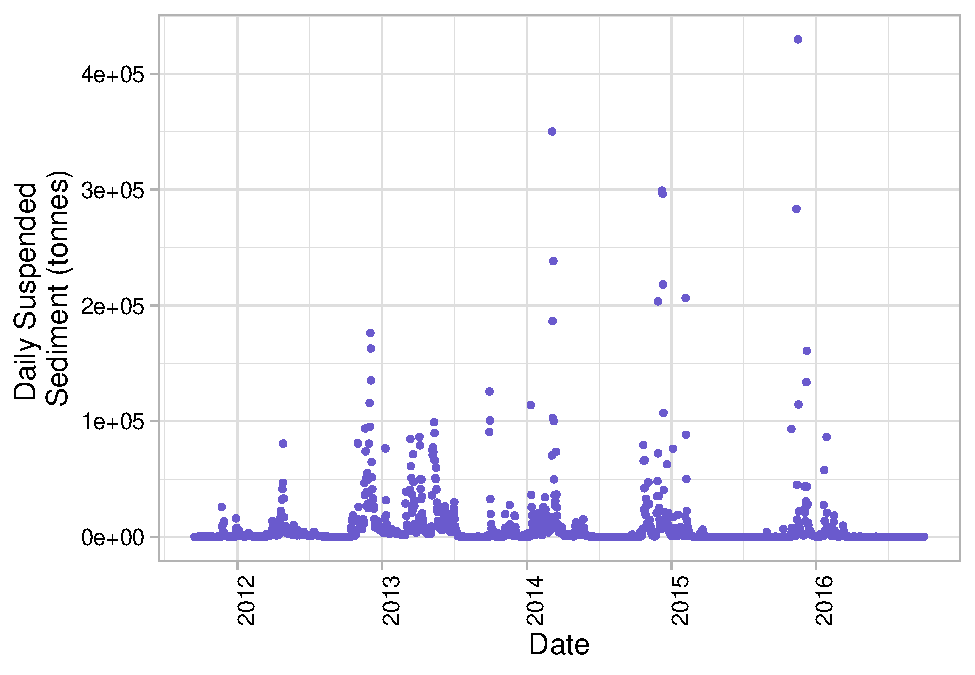
\includegraphics{Mason_ENV872_ProjectFinal_files/figure-latex/Exploratory Analysis Figure 2-1.pdf}
\caption{Daily suspended sediment in the Elwha River, WA, from September
15, 2011 to September 30, 2016.}
\end{figure}

\begin{figure}
\centering
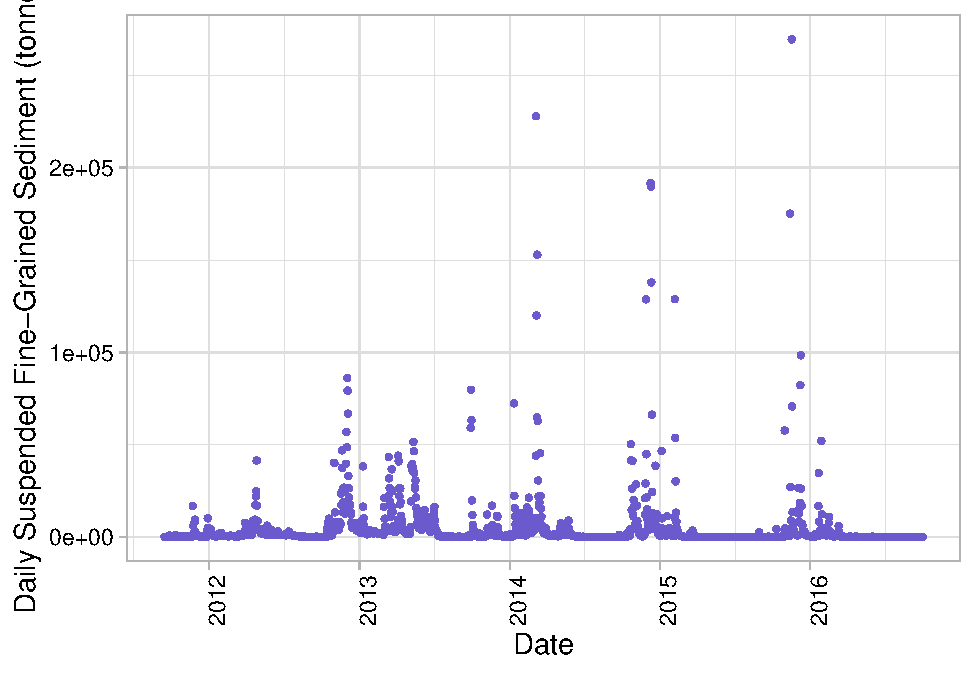
\includegraphics{Mason_ENV872_ProjectFinal_files/figure-latex/Exploratory Analysis Figure 3-1.pdf}
\caption{Daily suspended sediment of fine-grained particles in the Elwha
River, WA, from September 15, 2011 to September 30, 2016.}
\end{figure}

\begin{figure}
\centering
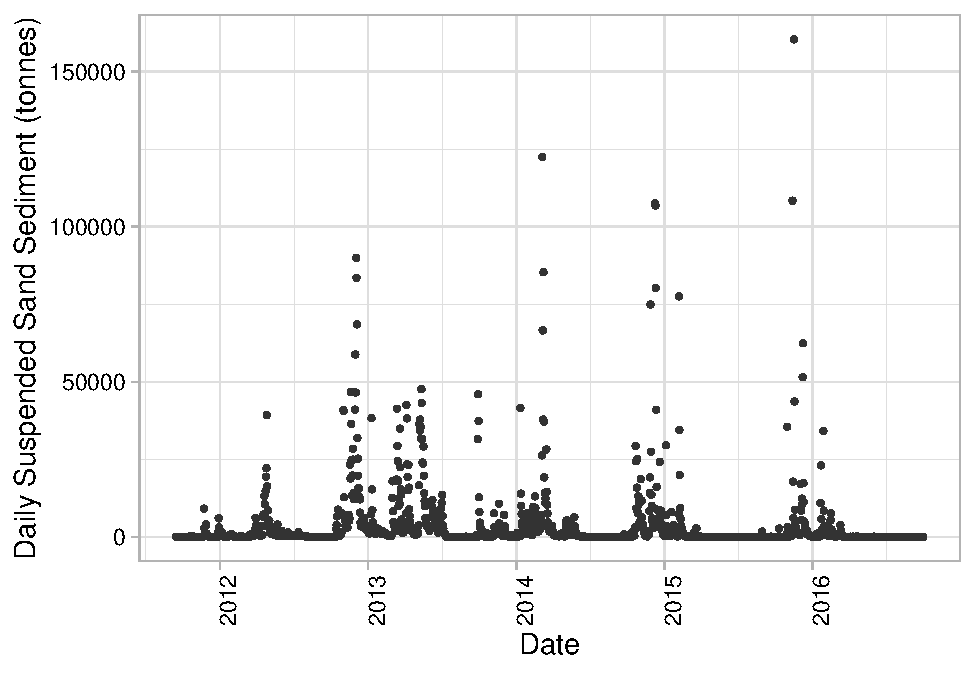
\includegraphics{Mason_ENV872_ProjectFinal_files/figure-latex/Exploratory Analysis Figure 4-1.pdf}
\caption{Daily suspended sediment of sand particles in the Elwha River,
WA, from September 15, 2011 to September 30, 2016.}
\end{figure}

\begin{figure}
\centering
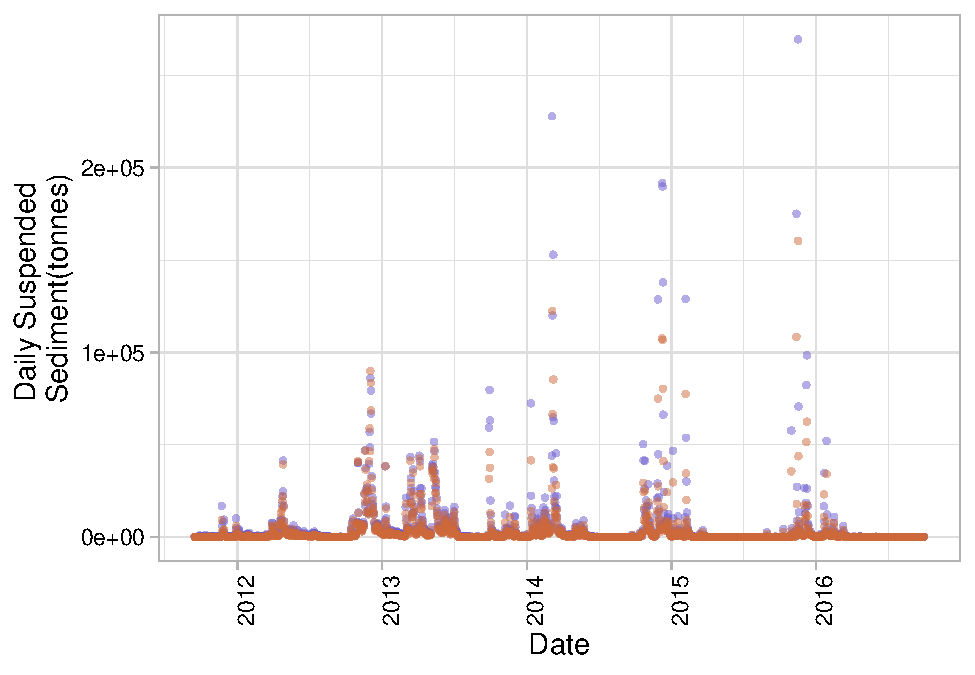
\includegraphics{Mason_ENV872_ProjectFinal_files/figure-latex/Exploratory Analysis Figure 5-1.pdf}
\caption{Daily suspended sediment of fine-grained particles (blue) and
sand particles (gray) in the Elwha River, WA, from September 15, 2011 to
September 30, 2016.}
\end{figure}

Suspended sediment concentrations might give a sense of the velocity of
the flow heading downstream, and how much sand was stuck behind the dams
that is then in movement after their removal. Looking at suspended
concentrations over time may show how long it takes for the sediment
behind the dam to resettle in the river, allowing the river to reach a
new morphological norm. General trends of suspended sediments,
\emph{Figure 2}, show more tonnes happening around the year 2013, which
is during the removal of the Elwha Dam, and the Glines Canyon Dam had
already been removed. However, there still exists some high recordings
of suspended sediment later on through the project years. However, these
might have to do with the high water discharge. Further analysis will
compare the relationship between daily suspended sediment and water
discharge over time. The dataset also has daily suspended sediment of
fine-grained particles, and sand particles. Their general point plots
are shown individually, \emph{Figures 3 and 4} and together in one plot,
\emph{Figure 5}, where we see there doesn't appear to be much difference
between the makeup of the suspended sediment, although a further test
can prove this.

\begin{figure}
\centering
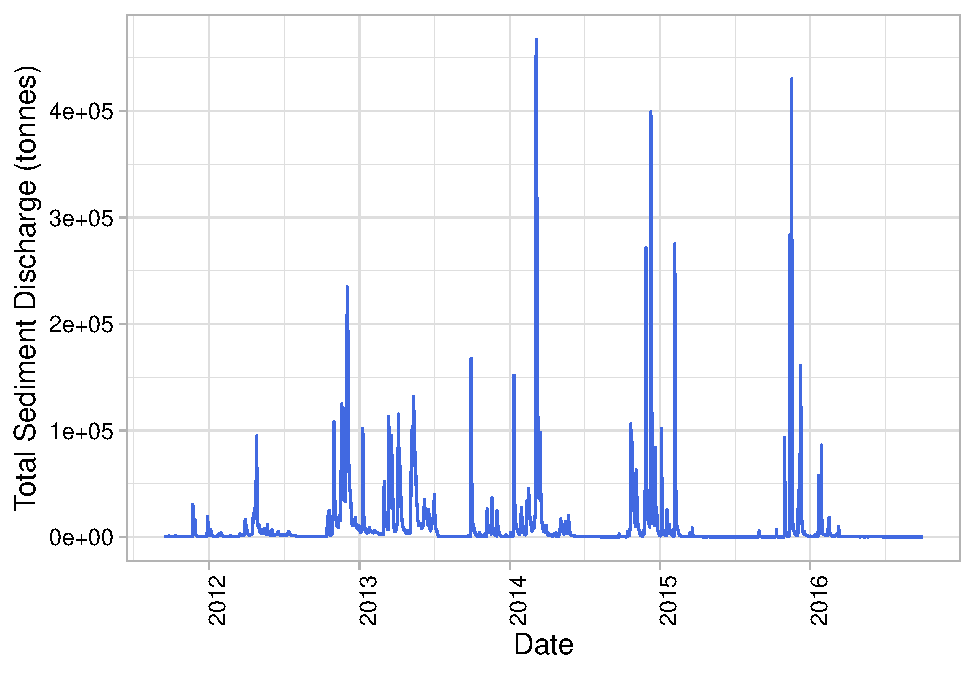
\includegraphics{Mason_ENV872_ProjectFinal_files/figure-latex/Exploratory Analysis Figure 6-1.pdf}
\caption{Daily total sediment discharge from the Elwha River, WA, from
September 15, 2011 to September 30, 2016.}
\end{figure}

\begin{figure}
\centering
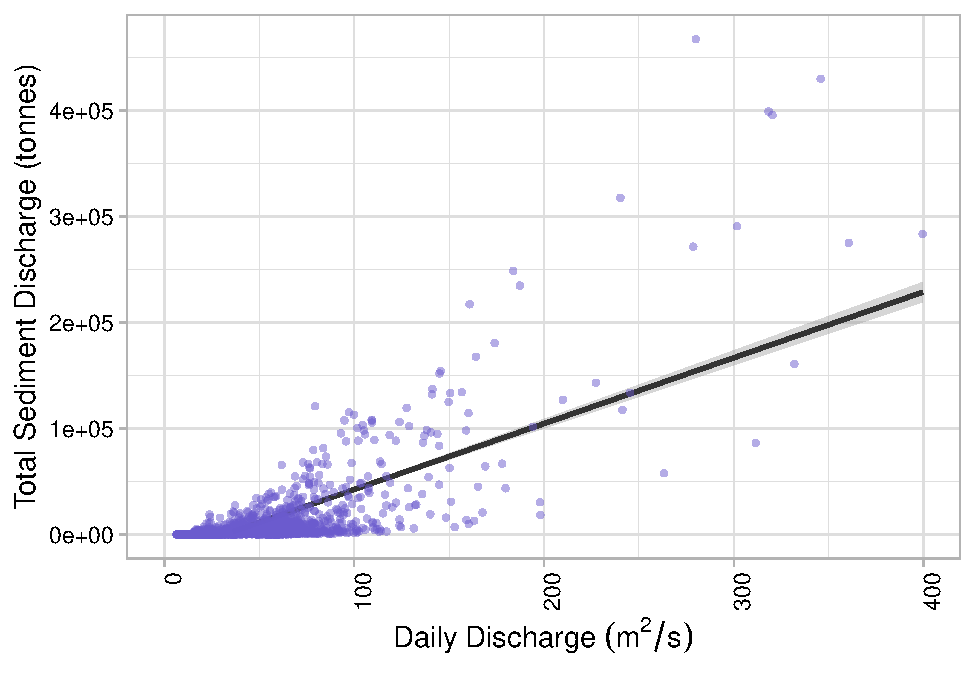
\includegraphics{Mason_ENV872_ProjectFinal_files/figure-latex/Exploratory Analysis Figure 7-1.pdf}
\caption{Daily total sediment discharge and water discharge on the Elwha
River, with a linear model, from September 15, 2011 to September 30,
2016.}
\end{figure}

While there are multiple parameters highlighting the sediment traveling
downstream, daily sediment discharge is a straight forward parameter of
moving sediment in the Elwha River during and after the dam removal
processes. From a general line plot of total sediment discharge over
time, \emph{Figure 6}, shows a peak discharge in 2013 and multiple large
peaks as well as what appears like a larger avergae sediment discharge
happening after 2014. These seem to make sense with the time stamps of
the dam removal process, but combining the time stamps and this
relationship in one graph will help better visualize the relationship
with dam removal over time. Calculations of yearly averages of total
sediment discharge will also be useful to determine if they are
increasing from 2012 to 2016 like they appear to be in this figure.

With daily water discharge and total sediment discharge being important
parameters for showing changes in the Elwha River following dam removal,
the relationship between them was graphed with a linear model to show a
relationship. It makes sense that increased flow would generate
increased sediment discharge, which we see from the positive linear
relationship. It would be interesting to see this relationship graphed
out for each individual year and see how this relationship might change.

\newpage

\hypertarget{analysis}{%
\section{Analysis}\label{analysis}}

\hypertarget{question-1-how-does-water-and-sediment-discharge-in-the-elwha-river-differ-during-and-after-the-two-part-dam-removal-process}{%
\subsection{Question 1: How does water and sediment discharge in the
Elwha River differ during and after the two part dam removal
process?}\label{question-1-how-does-water-and-sediment-discharge-in-the-elwha-river-differ-during-and-after-the-two-part-dam-removal-process}}

A closer look into total sediment discharge and daily discharge of water
from the Elwha River with attention on the time stamps of when the dam
removal project begigs, and when it is completed, \emph{Figures 8 and
9}, prompted an in depth analysis of trends. Data was separated into
during the dam removal process and after its completion, September 26,
2014.

\begin{figure}
\centering
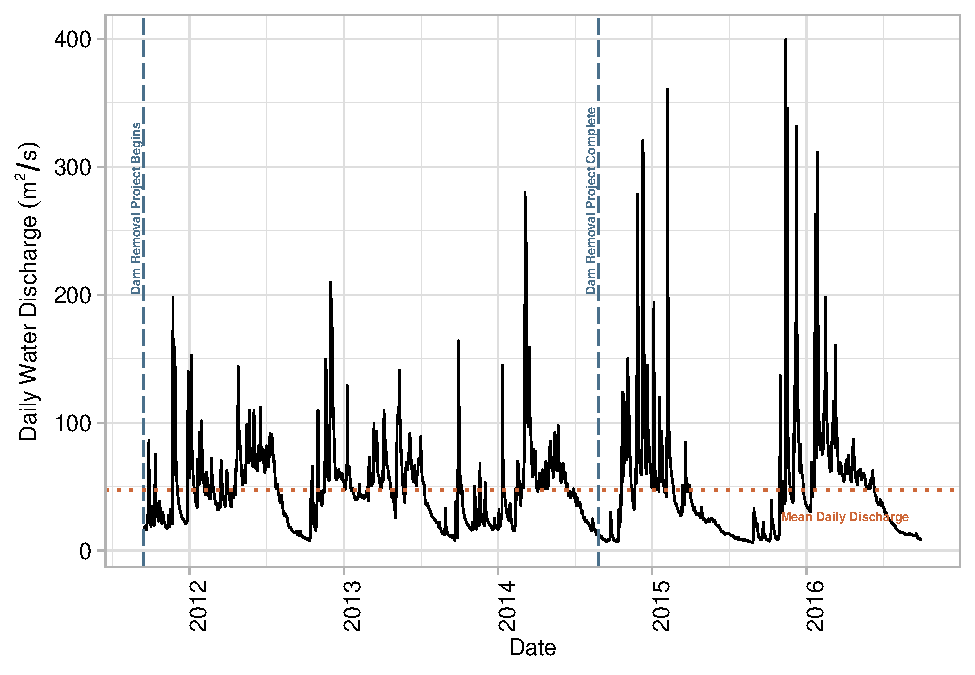
\includegraphics{Mason_ENV872_ProjectFinal_files/figure-latex/Intro to Question (Figure 8)-1.pdf}
\caption{Daily water discharge from the Elwha River from September 15,
2011 to September 30, 2016 measured at the U.S. Geological Survey gaging
station 12046260 at the diversion near Port Angeles, Washington. A
project to remove the Elwha and Glines Canyon Dam began on September 15,
2011, and was completed on August 26, 2014. Mean Daily discharge across
the whole time range was 47.7.}
\end{figure}

\begin{figure}
\centering
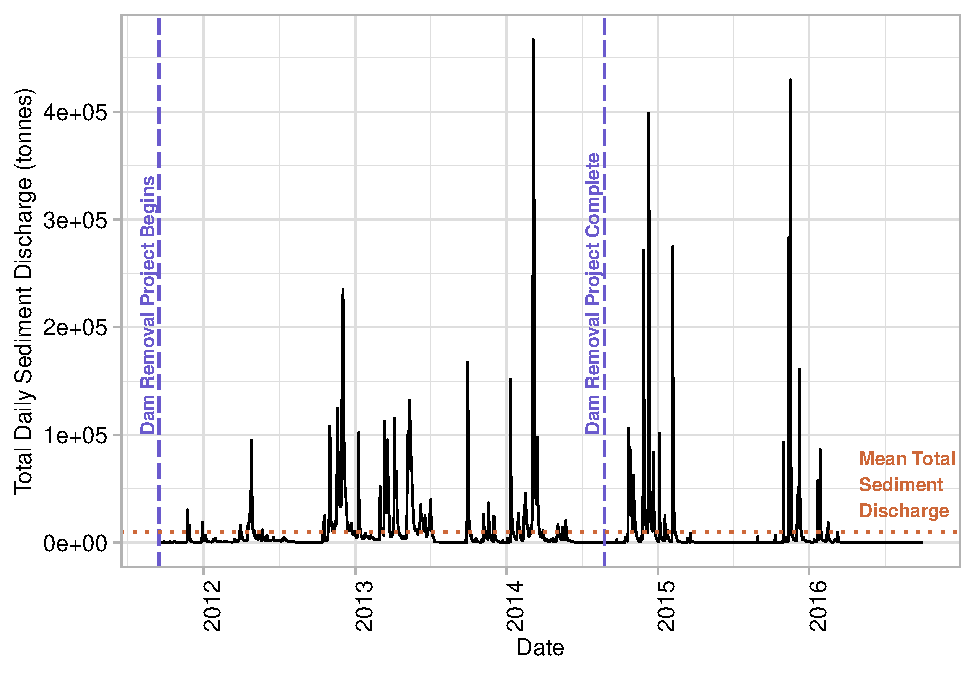
\includegraphics{Mason_ENV872_ProjectFinal_files/figure-latex/Intro to Question (Figure 9)-1.pdf}
\caption{Daily total sediment discharge from the Elwha River from
September 15, 2011 to September 30, 2016 measured at the U.S. Geological
Survey gaging station 12046260 at the diversion near Port Angeles,
Washington. A project to remove the Elwha and Glines Canyon Dam began on
September 15, 2011, and was completed on August 26, 2014. Mean Daily
sediment discharge across the whole time range was 9886.876 tonnes.}
\end{figure}

A two sample t-test revealed\ldots{}

\begin{figure}
\centering
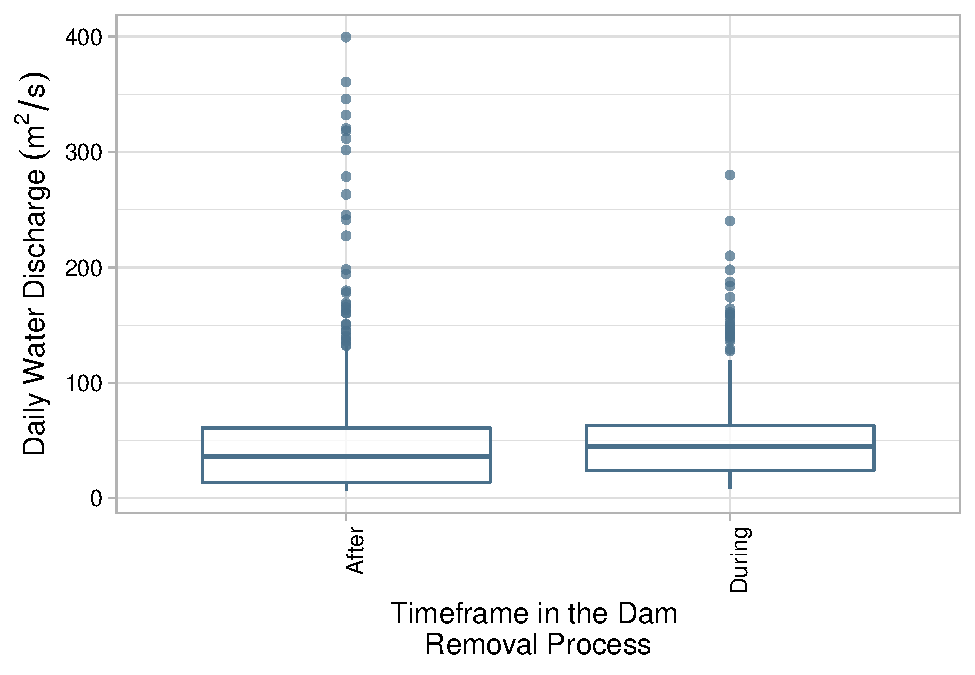
\includegraphics{Mason_ENV872_ProjectFinal_files/figure-latex/Two Way T-Test REsults Water (Figure 10)-1.pdf}
\caption{Daily water discharge distribution during and after the Elwha
River two dam removal process. During the dam removal is classified by
dates from September 15, 2011 to August 26, 2014, and after is from then
until September 30, 2016.}
\end{figure}

\begin{figure}
\centering
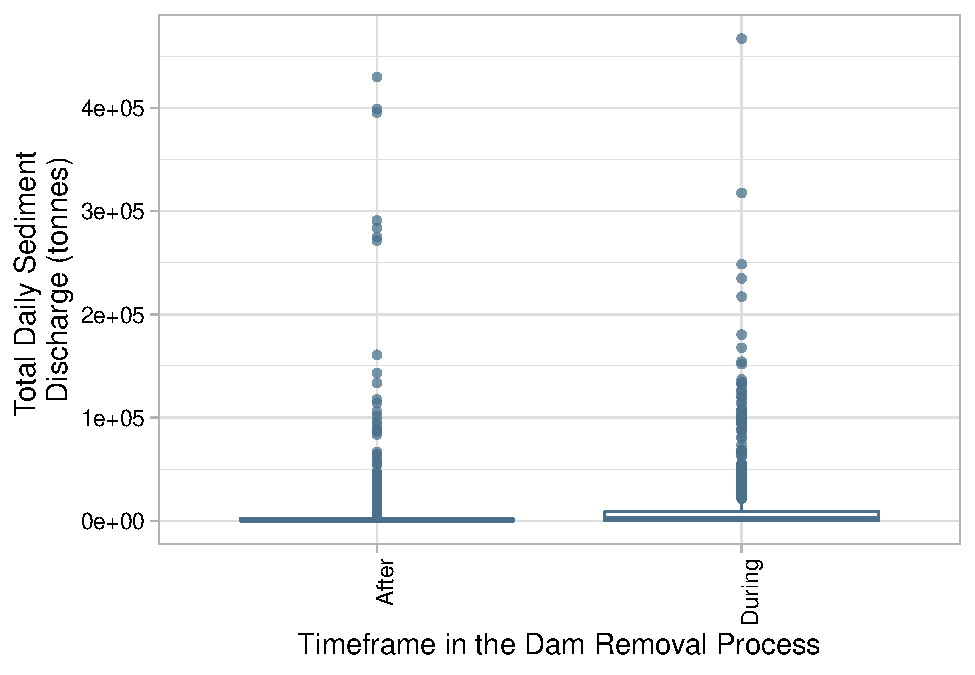
\includegraphics{Mason_ENV872_ProjectFinal_files/figure-latex/Two Way T-Test REsults sediment(Figure 11)-1.pdf}
\caption{Daily total sediment discharge distribution during and after
the Elwha River two dam removal process. During the dam removal is
classified by dates from September 15, 2011 to August 26, 2014, and
after is from then until September 30, 2016.}
\end{figure}

\newpage

\hypertarget{question-2-can-we-predict-sediment-discharge-from-water-flow-on-the-elwha-river}{%
\subsection{Question 2: Can we predict sediment discharge from water
flow on the Elwha
River?}\label{question-2-can-we-predict-sediment-discharge-from-water-flow-on-the-elwha-river}}

Increased water flow on a river should carry more sediment, producing
more overal sediment discharge. An analysis of water discharge and
sediment discharge is performed over the entirity of the sampling period
to find a general trend of the relationship of these two parameters over
time on the Elwha.

\begin{figure}
\centering
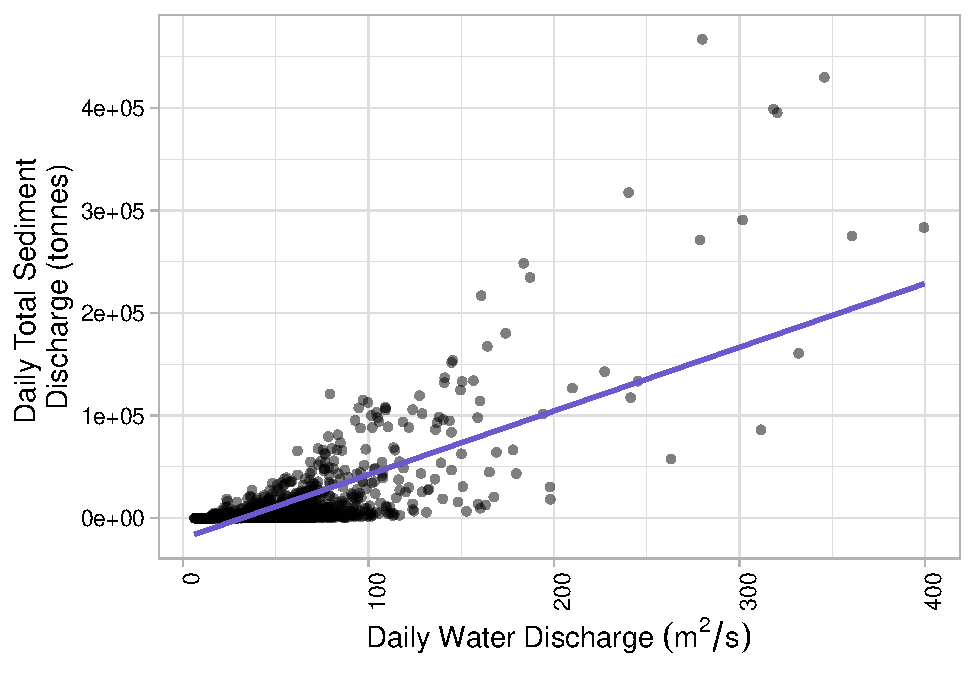
\includegraphics{Mason_ENV872_ProjectFinal_files/figure-latex/Linear Regression (figure 12)-1.pdf}
\caption{Daily water discharge as an indicator for daily total sediment
discharge on the Elwha River, with a linear regression.}
\end{figure}

A linear regression revealed\ldots{}

\#Question 2a: Does daily water discharge predict total sediment
discharge during and after the two part dam removal process?

\newpage

\hypertarget{summary-and-conclusions}{%
\section{Summary and Conclusions}\label{summary-and-conclusions}}

\newpage

\hypertarget{references}{%
\section{References}\label{references}}

\textless{}add references here if relevant, otherwise delete this
section\textgreater{}

\end{document}
